\documentclass[11pt]{article}
\usepackage[noend]{algpseudocode}
\usepackage{algorithm}
\usepackage{graphicx}
\usepackage{float}
\usepackage{fixltx2e}
\usepackage{wrapfig}
\usepackage{geometry}
\newgeometry{vmargin={39mm}, hmargin={30mm,30mm}} 

\begin{document}

{\centering
  \large Solution for Home Assignment 3 (Theoretical part)\\
   Danis Alukaev BS19-02\\ \par
}
\renewcommand*\Call[2]{\textproc{#1}(#2)}
\bigbreak
\noindent $\textbf{3.1. Constructing B-tree}$.\\
\noindent Given a set of keys $K = \{9, 31, 42, 69, 2, 26, 34, 57, 76, 27, 58\}$. Our goal is to store these keys in the B-tree with a minimum degree $t=2$, which can be defined as follows:\\
1. Every node other than the root must contain at least $1$ key.\\
2. Every internal node other than the root has at least $2$ children.\\
3. Every node can contain at most $3$ keys.\\ 
4. Every internal node can have at most $4$ children. \\
The resultant B-tree shown in Figure 1. Since the maximum degree (branch factor B) is even, we can implement an insert with a single pass down the tree (Preemptive splitting). 

\begin{figure}[h]
\centering
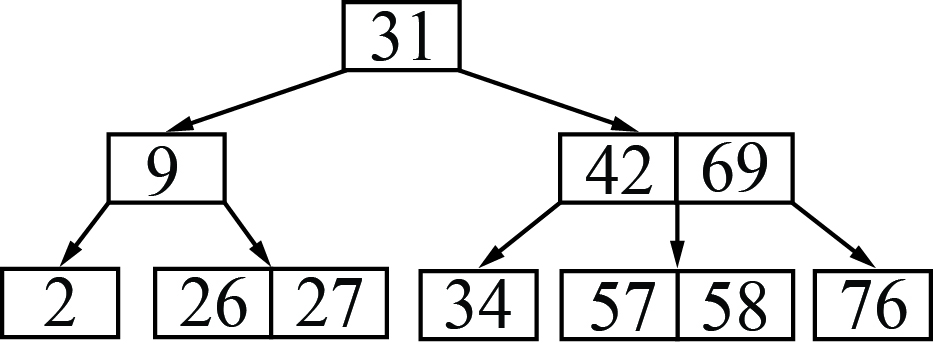
\includegraphics[width=0.35\linewidth]{DSA_1.jpg}
\caption{Resultant B-tree.}
\label{fig:mpr}
\end{figure}

\noindent Figure 2 provides the structures of the B-tree after each insertion indexed from 1 to 11 for a given set of keys.

\begin{figure}[h]
\centering
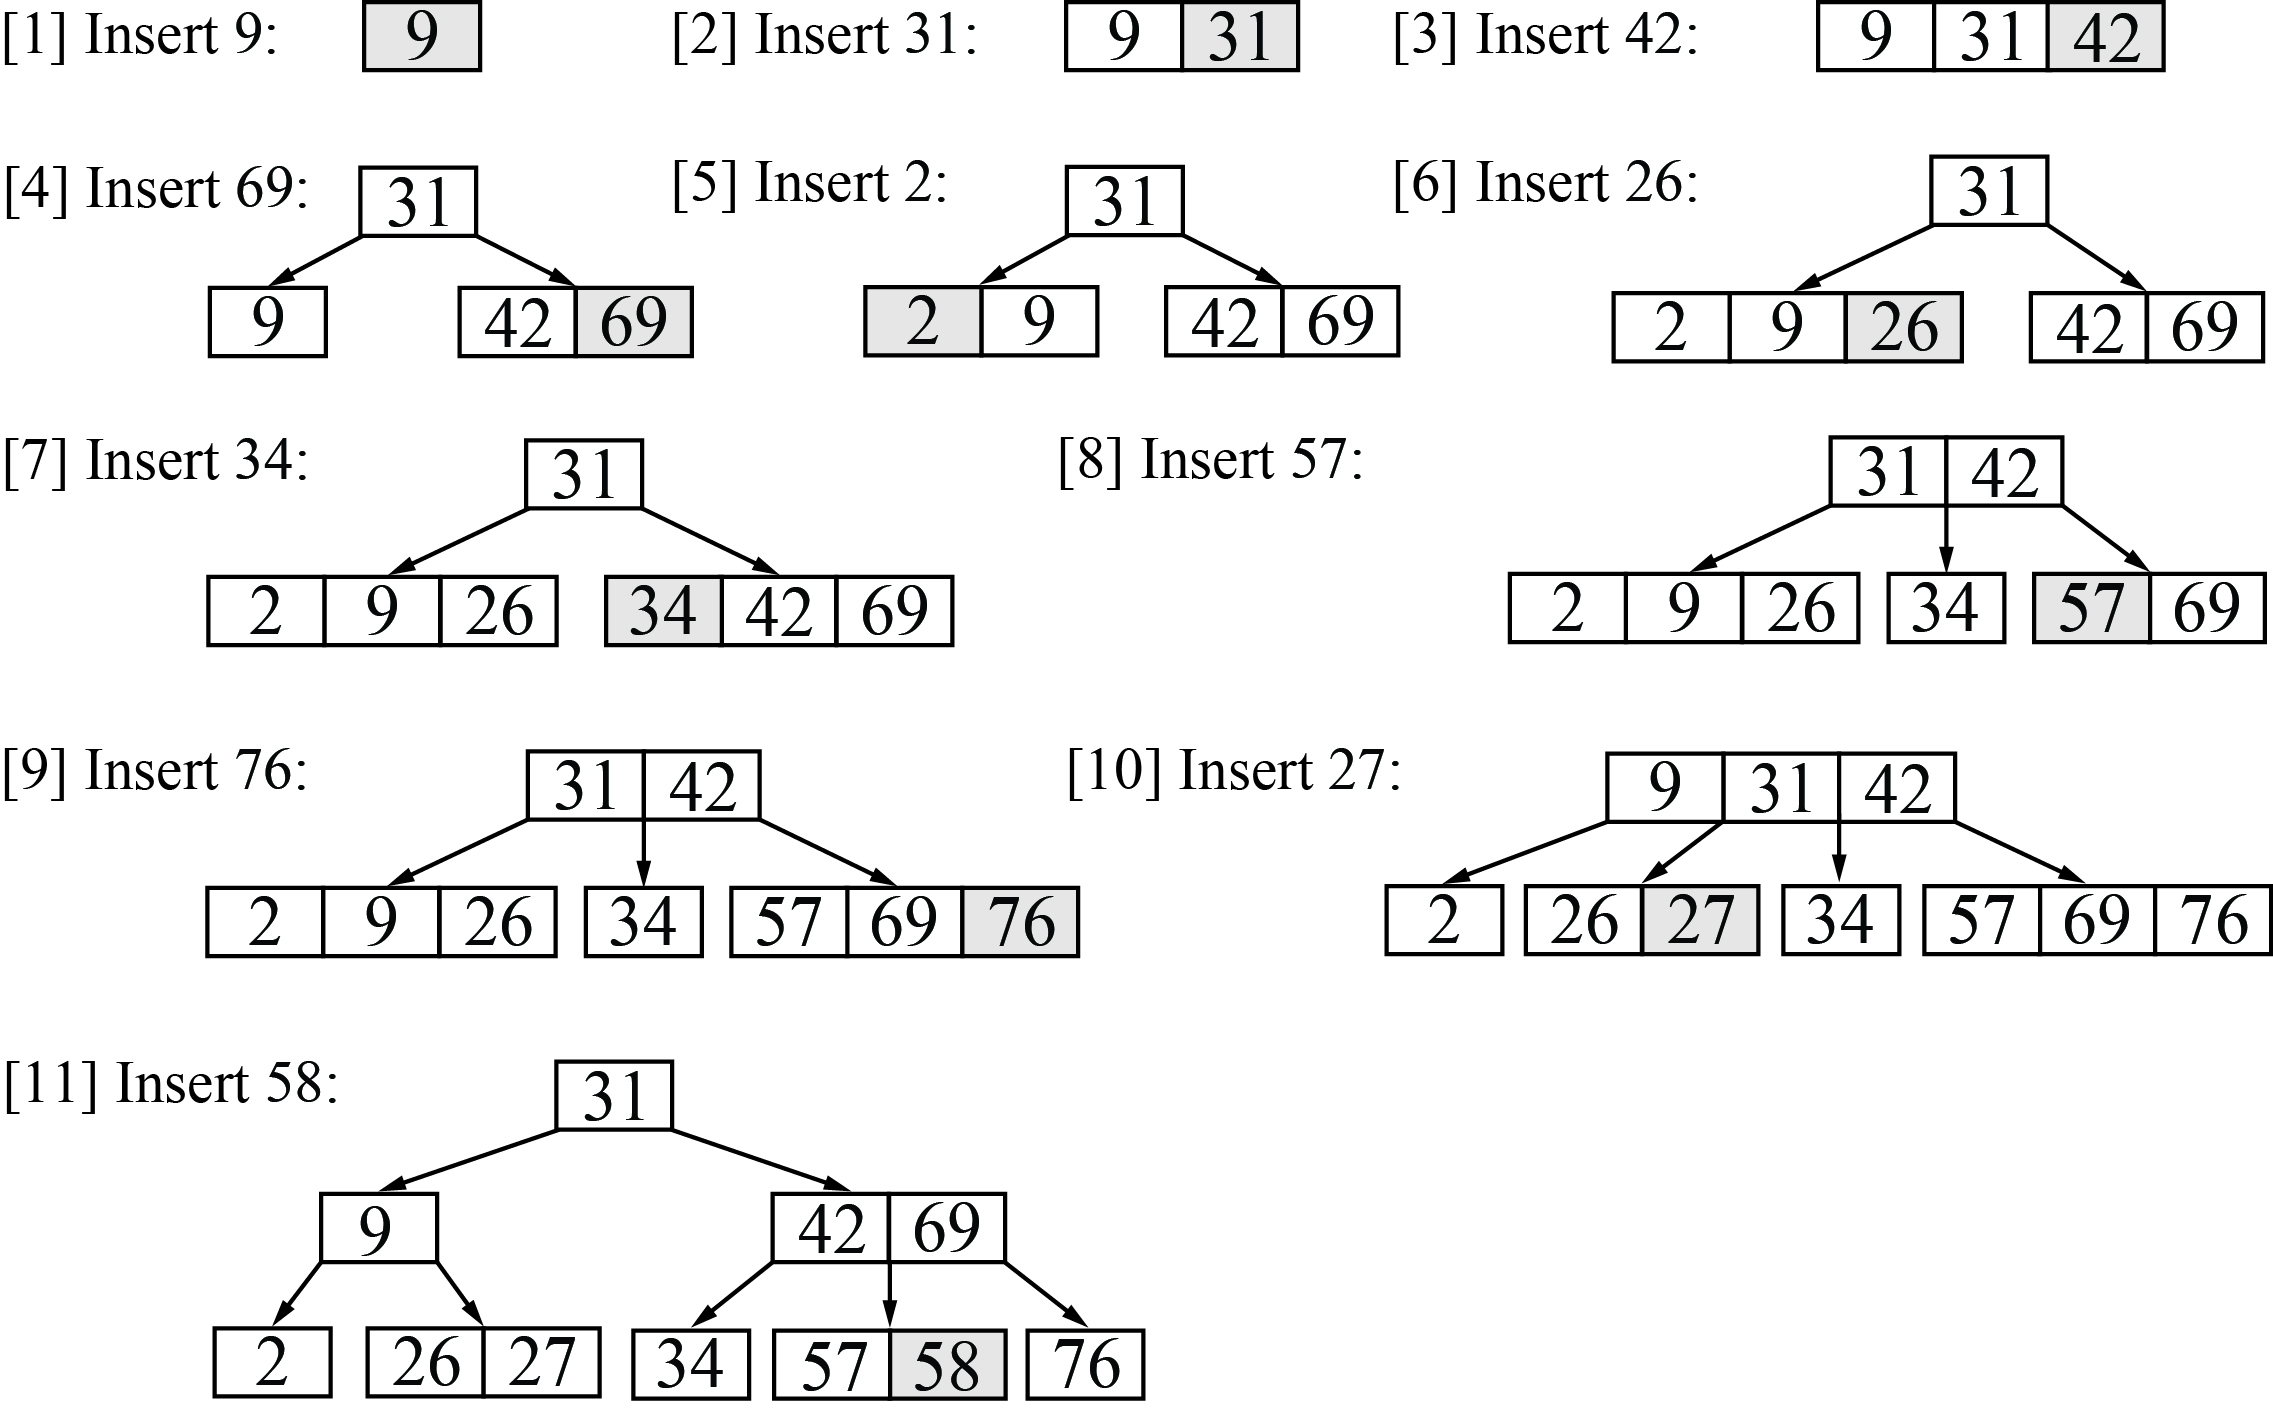
\includegraphics[width=0.85\linewidth]{DSA_2.jpg}
\caption{Inserting in B-tree.}
\label{fig:mpr}
\end{figure}

\noindent $\textbf{3.2. The square graph}$.\\

\noindent The square of a directed unweighted graph $G = (V, E)$ is the graph $G_{2} = (V, E_{2})$ such that $(u, w) \in E_{2}$ iff there exists $v \in V$ such that $(u, v) \in E$ and $(v, w) \in E$; i.e., there is a path of exactly two edges from $u$ to $w$. Our goal is to propose algorithms and their respective time complexities using the Big-O notation for constructing the square unweighted graphs.
\\ 
\\
\noindent The idea is to invoke the BFS and discover all vertices that are at distance of 2 from the starting vertex. Each of these vertices should be added to the adjacency list of starting vertex (or the connectivity marked in an adjacency matrix). Distance can be found using predecessor field $\pi$ of vertex (see Algorithm 1, 2). Proposed procedure repeated for all vertices of the graph. 
\\

\noindent The pseudocode of an algorithm for constructing the square graph using adjacency list shown in table Algorithm 1 (page 3). During the breadth-first search of an input graph $G(V, E)$, each vertex is enqueued and dequeued at most once. These operations take $O(1)$ time, so the total time devoted to process all vertices is $O(|V|)$. When vertex is dequeued an algorithm scans the corresponding adjacency list. The total sum of the lengths of all adjacency lists is $\Theta(|E|)$, so BFS requires $O(|E|)$ time to process all adjacency lists. Thus, the total running time of the BFS procedure is $O(|V|)+O(|E|)=O(|V|+|E|)$. The BFS is invoked for all vertices (to explore adjacent vertices at the distance of 2). Therefore, the time complexity of the proposed algorithm is $O(|V|(|V|+|E|))=O(|V|^{2}+|V||E|)=O(|V||E|)$. It is important to note that the worst case is $O(|V|^{3})$, because the number of edges in dense graphs is $E=\Theta(|V|^{2})$.
\\

\noindent The pseudocode of an algorithm for constructing the square graph using adjacency matrix shown in table Algorithm 2 (page 4). The total time devoted to enqueue-dequeue all vertices is the same with the Algorithm 1 and equals $O(|V|)$. However, when the vertex is dequeued an algorithm scans \textbf{all} the vertices (except dequeued one) of the graph to find adjacent vertices. The total number of these scans (all possible edges) is $\Theta(|V|^{2})$, so BFS requires $O(|V|^{2})$ time to determine all possible adjacent vertices. Thus, the total running time of the BFS procedure is $O(|V|)+O(|V|^{2})=O(|V|+|V|^{2})=O(|V|^{2})$. We repeat this procedure on all vertices of the graph, so the time complexity of the proposed algorithm is $O(|V|(|V|^{2}))=O(|V|^{3})$.



\begin{algorithm}
\caption{Algorithm for constructing the square graph (using adjacency list).}
\begin{algorithmic}[1]
\Procedure{Get}{$G.AdjList,v$}
\State \textbf{return} list of adjacent to a vertex $v$ vertices in a graph $G$
\EndProcedure
\Statex
\Procedure{Append}{$L,v$}
\State \textbf{add} the item $v$ to the end of the list $L$ 
\EndProcedure
\Statex
\Procedure{Square-Matrix}{$G$}
\State new \textbf{graph} $G_{2}$
\Comment create new graph $G_{2}$ 
\State $G_{2}.Vertices \gets G.Vertices$ \Comment copy the set of vertices
\State $G_{2}.AdjList \gets G.AdjList$  \Comment copy adjacency list
\For {each vertex $s$ $\in$ $G.Vertices$}
\State terminateBFS $\gets$ $False$ 
\For {each vertex $u$ $\in$ $G.Vertices$ – $\{s\}$} \Comment for all vertices except $s$
\State $u.state$ $\gets$ NOT VISITED \Comment set states and predecessors 
\State $u.\pi$ $\gets$ NIL 
\EndFor
\State $s.state$ $\gets$ OPENED \Comment mark $s$ as opened 
\State $s.\pi$ $\gets$ NIL \Comment mark predecessor as undefined
\State $Q$ $\gets$ $\emptyset$ \Comment create queue for BFS
\State \Call{Enqueue}{$Q,s$} 
\While{$Q$ $\neq$ $\emptyset$ and \textbf{not} terminateBFS}  
\State $u$ $\gets$ \Call{Dequeue}{Q} 
\For {each $v$ $\in$ \Call{Get}{$G.AdjList$, $u$}}
\Comment for all adjacent to $u$ vertices
\If {$v.state$ == NOT VISITED}
\State $v.state$ $\gets$ OPENED  
\State $v.\pi$ $\gets$ $u$ 
\State \Call{Enqueue}{$Q,v$} 
\If {$v.\pi.\pi$  == $s$} \Comment $v$ is at distance of 2 from starting $s$
\State \Call {Append}{\Call{Get}{$G_{2}.AdjList,s$}, $v$} \Comment insert new edge
\ElsIf {$v.\pi.\pi.\pi$  == $s$}\Comment $v$ is at distance of 3 from $s$
\State terminateBFS $\gets$ $True$ \Comment all vertices at distance of 2 are visited
\State \textbf{break} \Comment terminate BFS for $s$
\EndIf
\EndIf
\State $u.state$ $\gets$ EXITED \Comment mark vertex $u$ as exited
\EndFor
\EndWhile
\EndFor
\State \textbf{return} $G_{2}$
\EndProcedure
\end{algorithmic}
\end{algorithm}

\begin{algorithm}
\caption{Algorithm for constructing the square graph (using adjacency list).}
\begin{algorithmic}[1]
\Procedure{GetIndex}{$G,v$}
\State \textbf{return} index of vertex $v$ of a graph $G$ in adjacency matrix
\EndProcedure
\Statex
\Procedure{GetVertex}{$G,i$}
\State \textbf{return} vertex with index $i$ in adjacency matrix of a graph $G$ 
\EndProcedure
\Statex
\Procedure{Square-Matrix}{$G$}
\State new \textbf{graph} $G_{2}$ \Comment create new graph $G_{2}$ 
\State $G_{2}.Vertices \gets G.Vertices$ \Comment copy the set of vertices
\State $G_{2}.AdjMatrix \gets G.AdjMatrix$ \Comment copy adjacency matrix   
\For {each vertex $s$ $\in$ $G.Vertices$}
\State terminateBFS $\gets$ $False$
\For {each vertex $u$ $\in$ $G.Vertices$ – $\{s\}$} \Comment for all vertices except $s$
\State $u.state$ $\gets$ NOT VISITED \Comment set states and predecessors 
\State $u.\pi$ $\gets$ NIL 
\EndFor
\State $s.state$ $\gets$ OPENED \Comment mark $s$ as opened
\State $s.\pi$ $\gets$ NIL  \Comment mark predecessor as undefined
\State $Q$ $\gets$ $\emptyset$ \Comment create queue for BFS
\State \Call{Enqueue}{$Q,s$} 
\State $index_{s} \gets $ \Call {GetIndex}{$G,s$} \Comment find the index of $s$ in adjacency matrix
\While{$Q$ $\neq$ $\emptyset$ and \textbf{not} terminateBFS}  
\State $u$ $\gets$ \Call{Dequeue}{Q} 
\State $index_{u} \gets$ \Call{GetIndex}{$G,u$} \Comment find index of $u$ in adjacency matrix
\For {$i=0$ to $n$} \Comment treat all indexes of vertices in adjacency matrix
\If {$G.AdjMatrix$[$index_{u}][i] == 1$} \Comment check presence of edge
\State $v \gets$ \Call{GetVertex}{$G,i$} 
\If {$v.state$ == NOT VISITED}
\State $v.state$ $\gets$ OPENED 
\State $v.\pi$ $\gets$ $u$ 
\State \Call {Enqueue}{$Q,v$} 
\If {$v.\pi.\pi$  == $s$} \Comment $v$ is at distance of 2 from starting $s$
\State $G_{2}.AdjMatrix$[$index_{s}][i] \gets 1$ \Comment insert new edge
\ElsIf {$v.\pi.\pi.\pi$  == $s$} \Comment $v$ is at distance of 3 from $s$
\State terminateBFS $\gets$ $True$ \Comment all vertices at distance of 2 are visited
\State \textbf{break} \Comment terminate BFS for $s$
\EndIf
\EndIf
\EndIf
\State $u.state$ $\gets$ EXITED \Comment mark vertex $u$ as exited
\EndFor
\EndWhile
\EndFor
\State \textbf{return} $G_{2}$
\EndProcedure
\end{algorithmic}
\end{algorithm}

\end{document}